\subsection{Spectra}\label{sec:spectra}
%schriste - this section needs major work
%ji - there is no example of a spectrum
%dps - I need to think in one...
%schriste - can't we just take a slice off of the spectram to make a spectrum?
%dps - Spectrum does not really do much, just peek and plot. I don't think
% it brings anything to the content.
SunPy aims to provide broad support for solar spectroscopy
instruments.  The variety and complexity of these instruments and
their resultant datasets makes this a challenging goal.  The \texttt{spectra} module implements a
\texttt{Spectrum} class for 1D data (intensity as a function of frequency) and a
\texttt{Spectrogram} class for 2D data (intensity as a function of time and
frequency).  Each of these classes use a \texttt{numpy.ndarray} class
as its \texttt{data} attribute.  These two classes were implemented
by funding provided by the Astrophysics Research Group at Trinity
College Dublin, Ireland.

As with other SunPy data types, the \texttt{Spectrogram} class has been
built so that each instrument initialises using a subclass containing the instrument-specific 
functionalities. The common functionality provided by the base \texttt{Spectrogram} class includes
joining different time ranges and frequencies, performing frequency-dependent background subtraction,
and convenient visualization and sampling of the data.
Currently, the \texttt{Spectrogram} class supports radio spectrograms from the 
\href{http://www.e-callisto.org/}{e-Callisto}
solar radio spectrometer network and STEREO/SWAVES spectrograms.

Listing \ref{code:spectra} shows how the \texttt{CallistoSpectrogram}
object retrieves spectrogram data in the time range specified taken at
the observatory of interest.  When the data is requested using the
\texttt{from\_range()} function, the object merges all the downloaded
files into a single spectrogram, across time and frequency.
In the example shown, data is provided in two frequency ranges, 
20--90\,MHz and 55--355\,MHz.  Since the data is not evenly spaced in
the frequency range, the \texttt{Spectrogram} object linearises the
frequency axis for a better analysis.  The example also demonstrates
the implemented background subtraction method which it calculates
a constant background over time for each frequency channel based on 
the values closer to the average.
% RJH: Which subtraction method?  If the specifics are irrelevant, cut it.
% RJH: is this better?
%ji to DPS - what is the linearisation that is happening here?
%ji- the linearisation consist in the frequency axis being linear and the 
% data being streched with it.  The frequency normally are not evenly spaced

\begin{listing}[H]
\begin{minted}[bgcolor=bg]{pycon}
>>> from sunpy.spectra.sources.callisto import CallistoSpectrogram
>>> tstart, tend = "2011-06-07T06:00:00", "2011-06-07T07:45:00"
>>> callisto = CallistoSpectrogram.from_range("BIR", tstart, tend)
>>> callisto_nobg = callisto.subtract_bg()
>>> callisto_nobg.peek(vmin = 0)
\end{minted}
\begin{center}
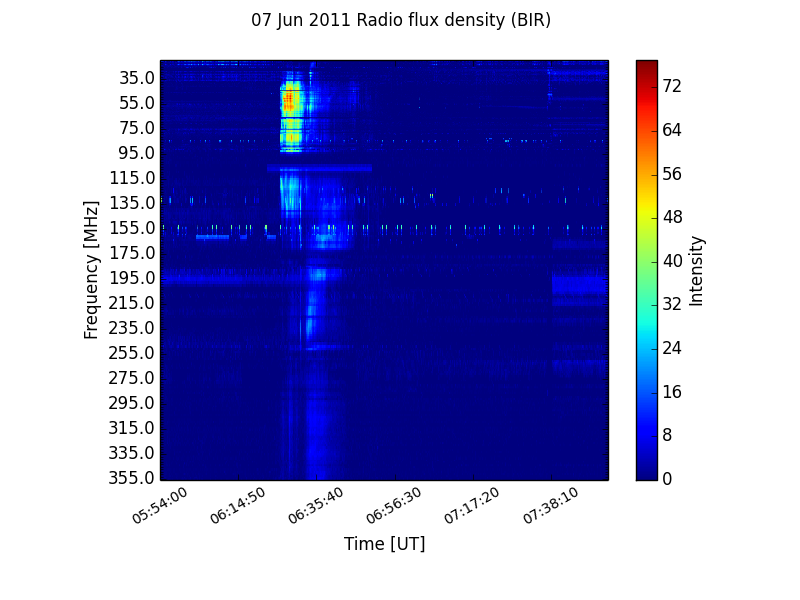
\includegraphics[width=0.8\columnwidth]{callisto_nobg}
\end{center}
\caption{Example of how \texttt{CallistoSpectrogram} retrieves the
  data for the requested time range and observatory, merges it and
  removes the background signal.  The data requested -- `BIR' -- is
  the code name of the \href{http://www.rosseobservatory.ie}{Rosse Observatory}
  at Birr Castle in Ireland.}
\label{code:spectra}
\end{listing}

